\documentclass[11pt]{article}

\usepackage[a4paper,margin=1in]{geometry}
\usepackage{amsmath,amssymb}
\usepackage{booktabs}
\usepackage{graphicx}
\usepackage[hypertexnames=false]{hyperref}
\usepackage{float}
\usepackage{siunitx}
\usepackage{enumitem}

\graphicspath{{figures/}{../Scripts/baseline_paper_reconstruction/outputs/}{../Scripts/non_markovian_extension/outputs/}{../Scripts/floquet_buffer_extension/outputs/}{../Scripts/thermodynamic_floquet_gate_prototype/outputs/}}

\title{Thermodynamic Quantum Logic with Floquet-Buffered Reservoir Coupling}
\author{Thermodynamic Quantum Gates Project}
\date{\today}

\begin{document}
\maketitle

\begin{abstract}
Autonomous quantum thermal machines provide a route to computation in which logical
states are encoded in thermodynamic variables and processed by heat currents rather than
externally clocked unitary gates.  We reconstruct the weak-coupling thermodynamic-neuron
model for NOT, NOR, majority, and XOR logic, using the virtual-temperature mechanism of
the baseline theory as the Markovian reference.  We then extend the numerical programme
toward structured reservoirs by validating a single-qubit non-Markovian benchmark and by
introducing a periodically driven Floquet buffer between a logical qubit and its bath.  The
buffer is assessed operationally through output-state distinguishability and an integrated
drive-work proxy.  In the present parameter set, the buffered architecture increases the
final trace distance from $0.1353$ to $0.1818$, while a broader screening sweep finds
positive distinguishability gain in $14$ of $15$ tested configurations.  These results support
a cautious next step: a minimal Floquet-buffered thermodynamic NOT prototype, before any
claim of a full multi-qubit non-Markovian thermal logic gate.
\end{abstract}

\section{Introduction}

Thermodynamic computing asks whether physical relaxation can be used directly as a
computational resource.  In the thermodynamic-neuron model, logical inputs are encoded as
inverse temperatures, a collector induces heat currents through a finite output reservoir,
and the final output inverse temperature is decoded as a logical value.  The main appeal of
this architecture is that computation is autonomous: the system relaxes toward a logical
answer without an externally prescribed sequence of gates.

The present work has two aims.  First, we reproduce the analytical Markovian
thermodynamic-neuron response of the baseline model, thereby establishing a reference for
logic fidelity and dissipation.  Second, we formulate the next extension: replacing ideal
memoryless reservoir contact by structured-bath dynamics, and testing whether a driven
Floquet buffer can improve output distinguishability before the logical subsystem loses
information to the environment.

\section{Markovian Thermodynamic-Neuron Model}

\subsection{Thermal Occupation and Virtual Temperature}

The elementary thermal nonlinearity is the two-level occupation
\begin{equation}
    g(\beta\epsilon)=\frac{1}{1+\exp(\beta\epsilon)} ,
    \label{eq:fermi}
\end{equation}
where $\epsilon$ is the qubit gap and $\beta$ is the inverse temperature.  For the
three-qubit collector used in the NOT gate, the relevant virtual inverse temperature is
\begin{equation}
    \beta_v
    =
    \frac{\epsilon_0}{\epsilon_z}\beta_0
    -
    \frac{\epsilon_1}{\epsilon_z}\beta_1,
    \qquad
    \epsilon_z=\epsilon_0-\epsilon_1 .
    \label{eq:virtual-temperature}
\end{equation}
Thus the input temperature $\beta_1$ controls the sign and magnitude of the effective
thermal bias seen by the output reservoir.

\subsection{Reset-Model Currents}

In the weak-coupling reset description, the collector and modulator currents are
\begin{align}
    j_C &=
    \mu\epsilon_z\left[g_z(\beta_z)-g_z(\beta_v)\right], \\
    j_M &=
    \mu'\epsilon_z\left[g_z(\beta_z)-g_z(\beta_r)\right],
\end{align}
with $g_z(\beta)=g(\beta\epsilon_z)$.  The finite output reservoir evolves according to
\begin{equation}
    \dot{\beta}_z(t)
    =
    -\frac{\beta_z(t)^2}{C}\left[j_C(t)+j_M(t)\right].
    \label{eq:beta-dynamics}
\end{equation}
The steady condition $j_C+j_M=0$ gives the bounded output $\beta_z^\infty$, which is the
decoded logical response.

\section{Baseline Logic Reconstruction}

The reconstructed Markovian response includes the virtual-temperature regimes, NOT
transfer curve, error--dissipation trade-off, NOR surface, three-input majority response,
and an XOR network assembled from thermodynamic-neuron subgates.  The role of this stage
is not merely illustrative; it fixes the baseline against which all non-Markovian or
Floquet-buffered extensions must be judged.

\begin{figure}[H]
    \centering
    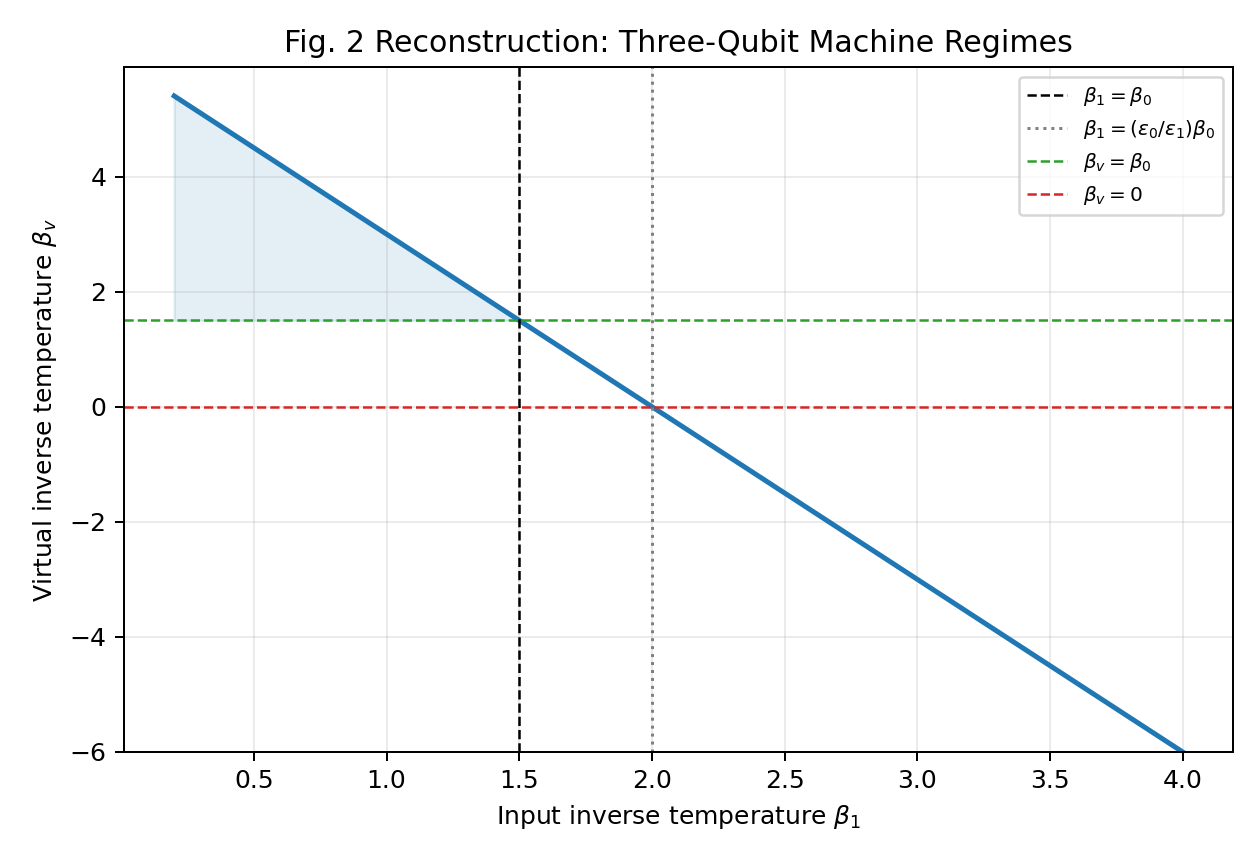
\includegraphics[width=0.74\linewidth]{fig2_virtual_temperature_regimes.png}
    \caption{Virtual-temperature regimes of the collector.  Sweeping the input inverse
    temperature changes the virtual thermal bias and therefore the direction in which the
    collector drives the finite output reservoir.}
    \label{fig:virtual-regimes}
\end{figure}

\begin{figure}[H]
    \centering
    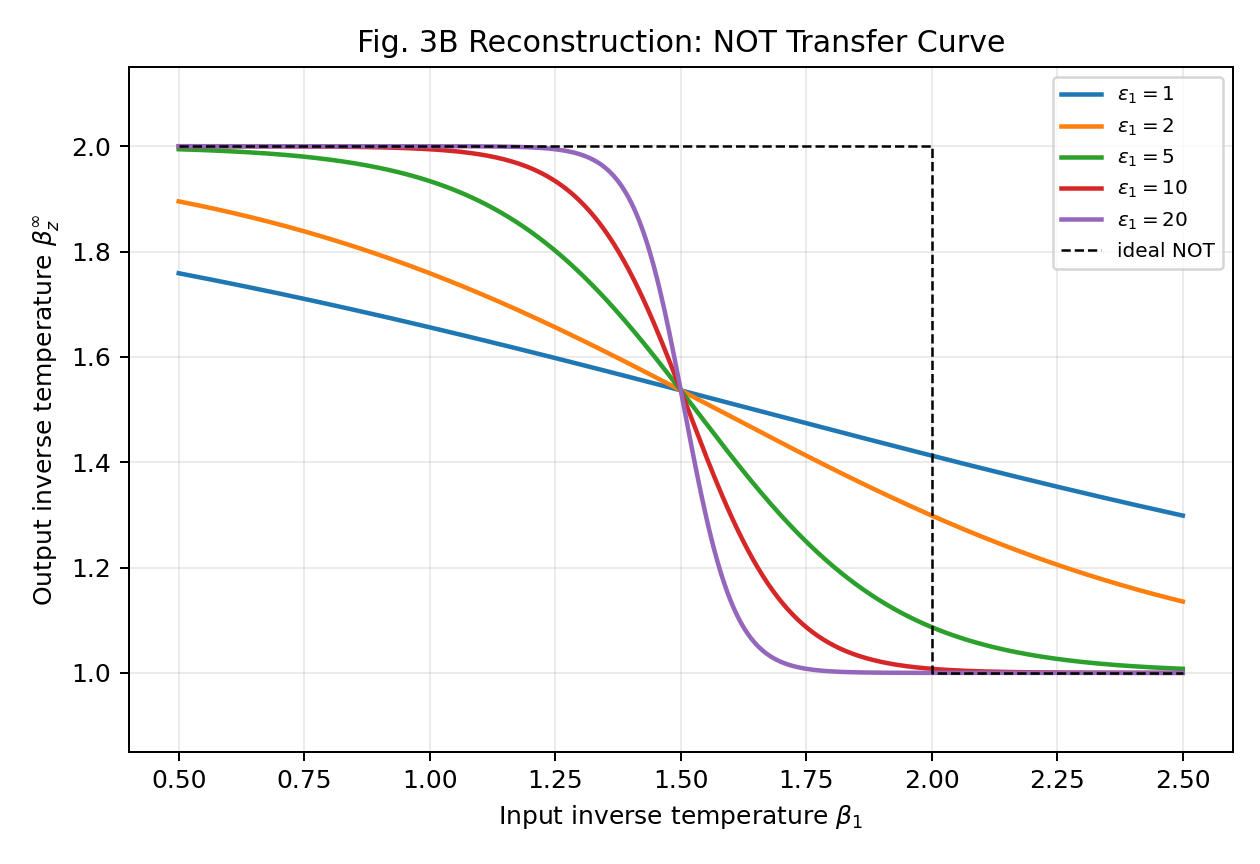
\includegraphics[width=0.74\linewidth]{fig3b_not_transfer_curve.png}
    \caption{Thermodynamic NOT response.  The steady output inverse temperature switches
    between the two logical temperature levels as the input inverse temperature is varied.
    Increasing the collector energy scale sharpens the transfer curve.}
    \label{fig:not-transfer}
\end{figure}

\begin{figure}[H]
    \centering
    
\includegraphics[width=0.74\linewidth]{fig3c_error_dissipation_tradeoff.png}
    \caption{Error--dissipation relation for the reconstructed NOT gate.  Larger energy
    scales suppress decoding error, but the entropy-production cost increases strongly.}
    \label{fig:error-dissipation}
\end{figure}

\begin{table}[H]
\centering
\caption{Representative error--dissipation data for increasing collector energy scale.}
\begin{tabular}{rrrr}
\toprule
$\epsilon_1$ & Average error & Average entropy production & Hot-input output \\
\midrule
1  & $1.6477\times 10^{-1}$ & $3.7266\times 10^{4}$ & 1.6561 \\
2  & $3.1114\times 10^{-2}$ & $2.8675\times 10^{5}$ & 1.7588 \\
5  & $2.1882\times 10^{-4}$ & $3.1029\times 10^{6}$ & 1.9338 \\
10 & $1.9770\times 10^{-5}$ & $9.5496\times 10^{6}$ & 1.9942 \\
20 & $1.5480\times 10^{-5}$ & $1.9882\times 10^{7}$ & 2.0000 \\
\bottomrule
\end{tabular}
\label{tab:error-dissipation}
\end{table}

\begin{figure}[H]
    \centering
    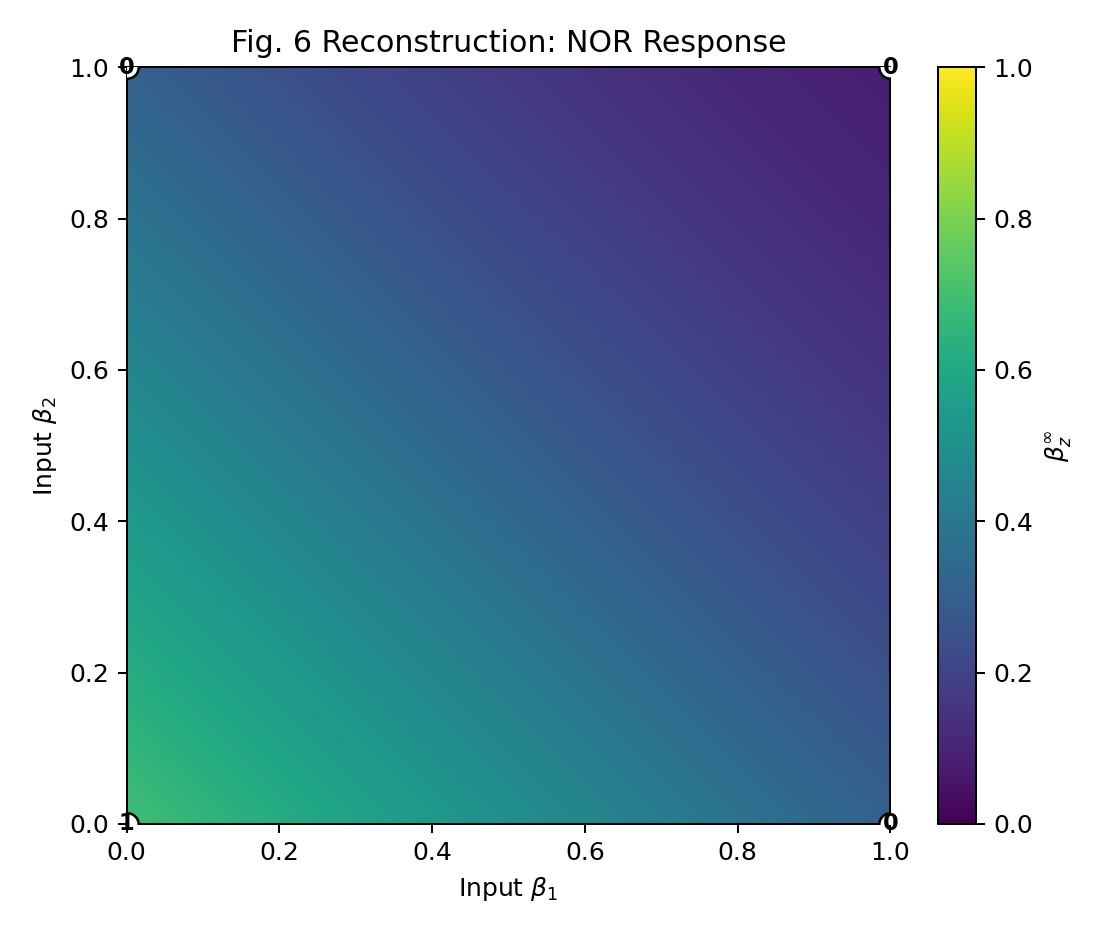
\includegraphics[width=0.74\linewidth]{fig6_nor_response_surface.png}
    \caption{Thermodynamic NOR response.  The high-output region occurs only near the
    low-low input corner, as required by NOR logic.}
    \label{fig:nor}
\end{figure}

\begin{figure}[H]
    \centering
    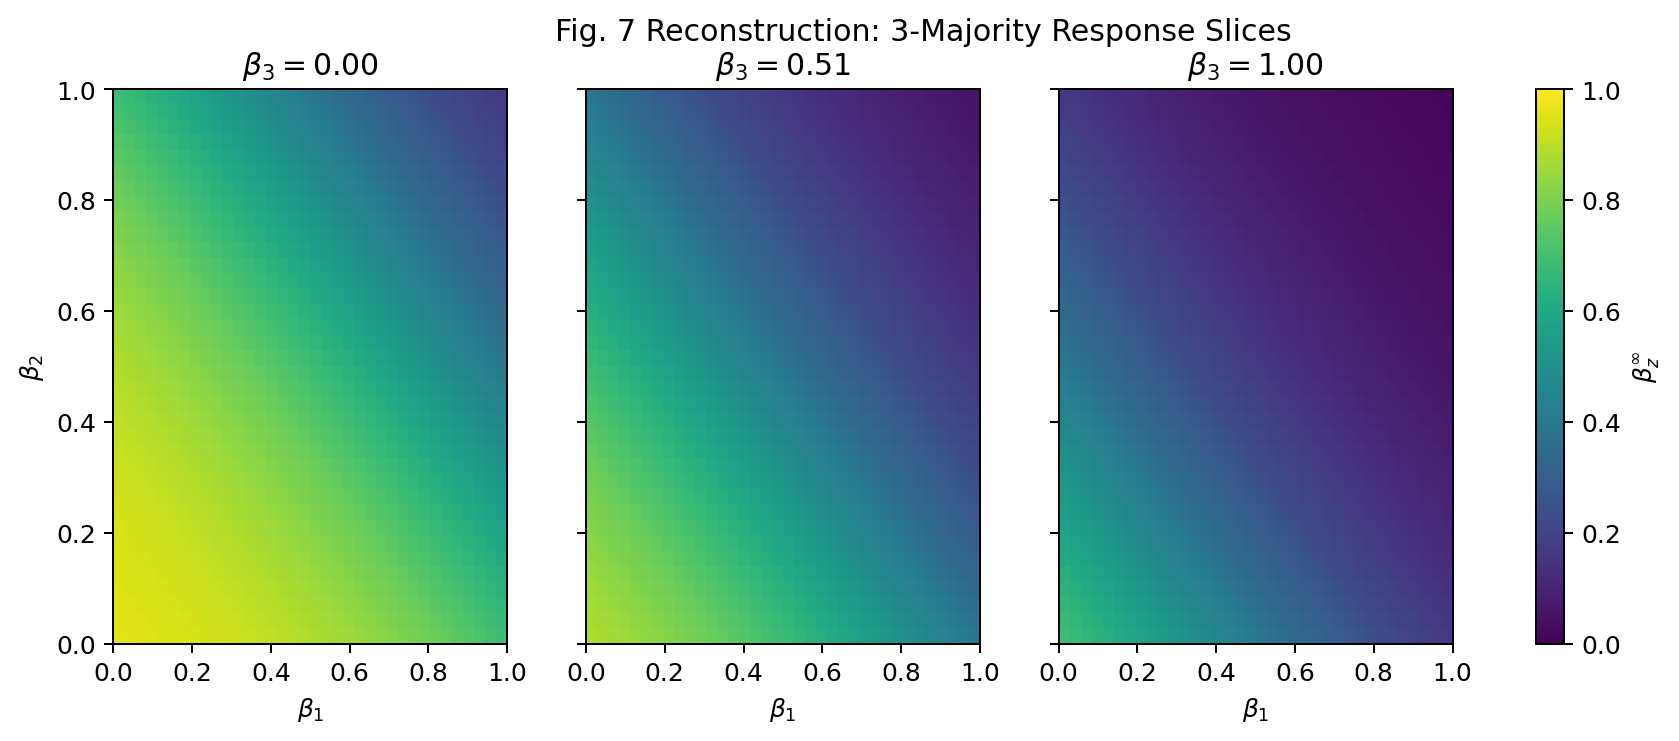
\includegraphics[width=0.74\linewidth]{fig7_majority_response_slices.png}
    \caption{Three-input majority response shown through two-dimensional slices.  The
    response is consistent with a thermodynamic perceptron whose virtual temperature is a
    linear score of the input temperatures.}
    \label{fig:majority}
\end{figure}

\begin{figure}[H]
    \centering
    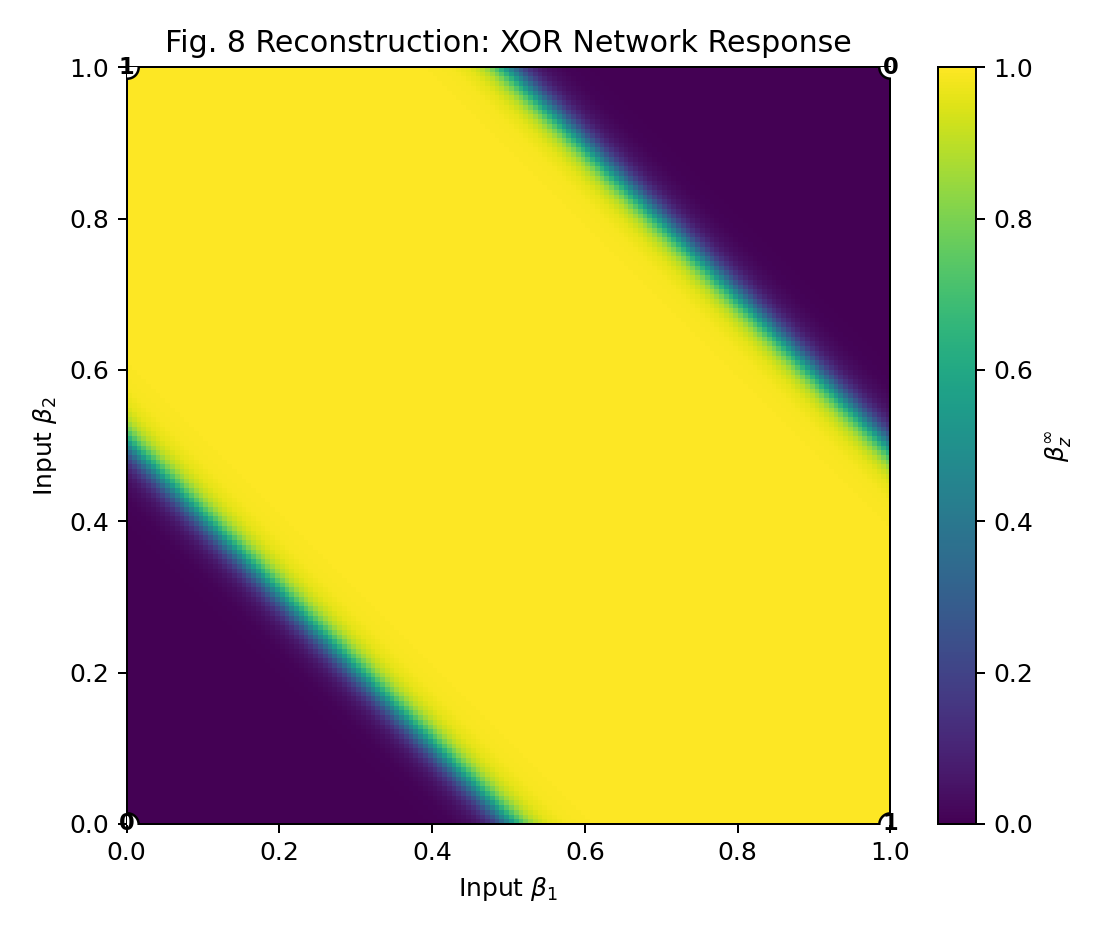
\includegraphics[width=0.74\linewidth]{fig8_xor_network_response.png}
    \caption{XOR response obtained by composing thermodynamic-neuron subgates.  Since XOR
    is not linearly separable, it is represented as a small network rather than a single
    perceptron.}
    \label{fig:xor}
\end{figure}

\section{Structured-Bath Benchmark}

A full thermodynamic gate under a structured reservoir should not be attempted before the
non-Markovian solver is numerically stable.  We therefore study a single qubit coupled to a
bosonic bath with spectral density
\begin{equation}
    J(\omega)=2\alpha\omega^s\exp(-\omega/\omega_c).
    \label{eq:spectral-density}
\end{equation}
The benchmark tracks trace preservation, Hermiticity, purity, and the final relaxation
observable across sub-Ohmic, Ohmic, and super-Ohmic regimes.

\begin{table}[H]
\centering
\caption{Single-qubit structured-bath benchmark.}
\begin{tabular}{lrrrr}
\toprule
Regime & $s$ & Final purity & Final $\sigma_z$ & Runtime (s) \\
\midrule
Sub-Ohmic & 0.5 & 0.5070 & -0.1184 & 20.996 \\
Ohmic & 1.0 & 0.5248 & 0.2230 & 6.582 \\
Super-Ohmic & 3.0 & 0.8421 & 0.8272 & 4.479 \\
\bottomrule
\end{tabular}
\label{tab:structured-bath}
\end{table}

The numerical-health checks are within the current tolerance: the largest trace deviation
is $1.884\times10^{-5}$ and the largest Hermiticity error is $5.011\times10^{-7}$.  Separate
time-step and memory-time scans pass a $10^{-3}$ final-observable tolerance.  The practical
working point for the next stage is
\begin{equation}
    dt=0.05,\qquad
    t_{\mathrm{mem}}=1.0,\qquad
    \chi_{\mathrm{svd}}=10^{-6}.
\end{equation}

\begin{figure}[H]
    \centering
    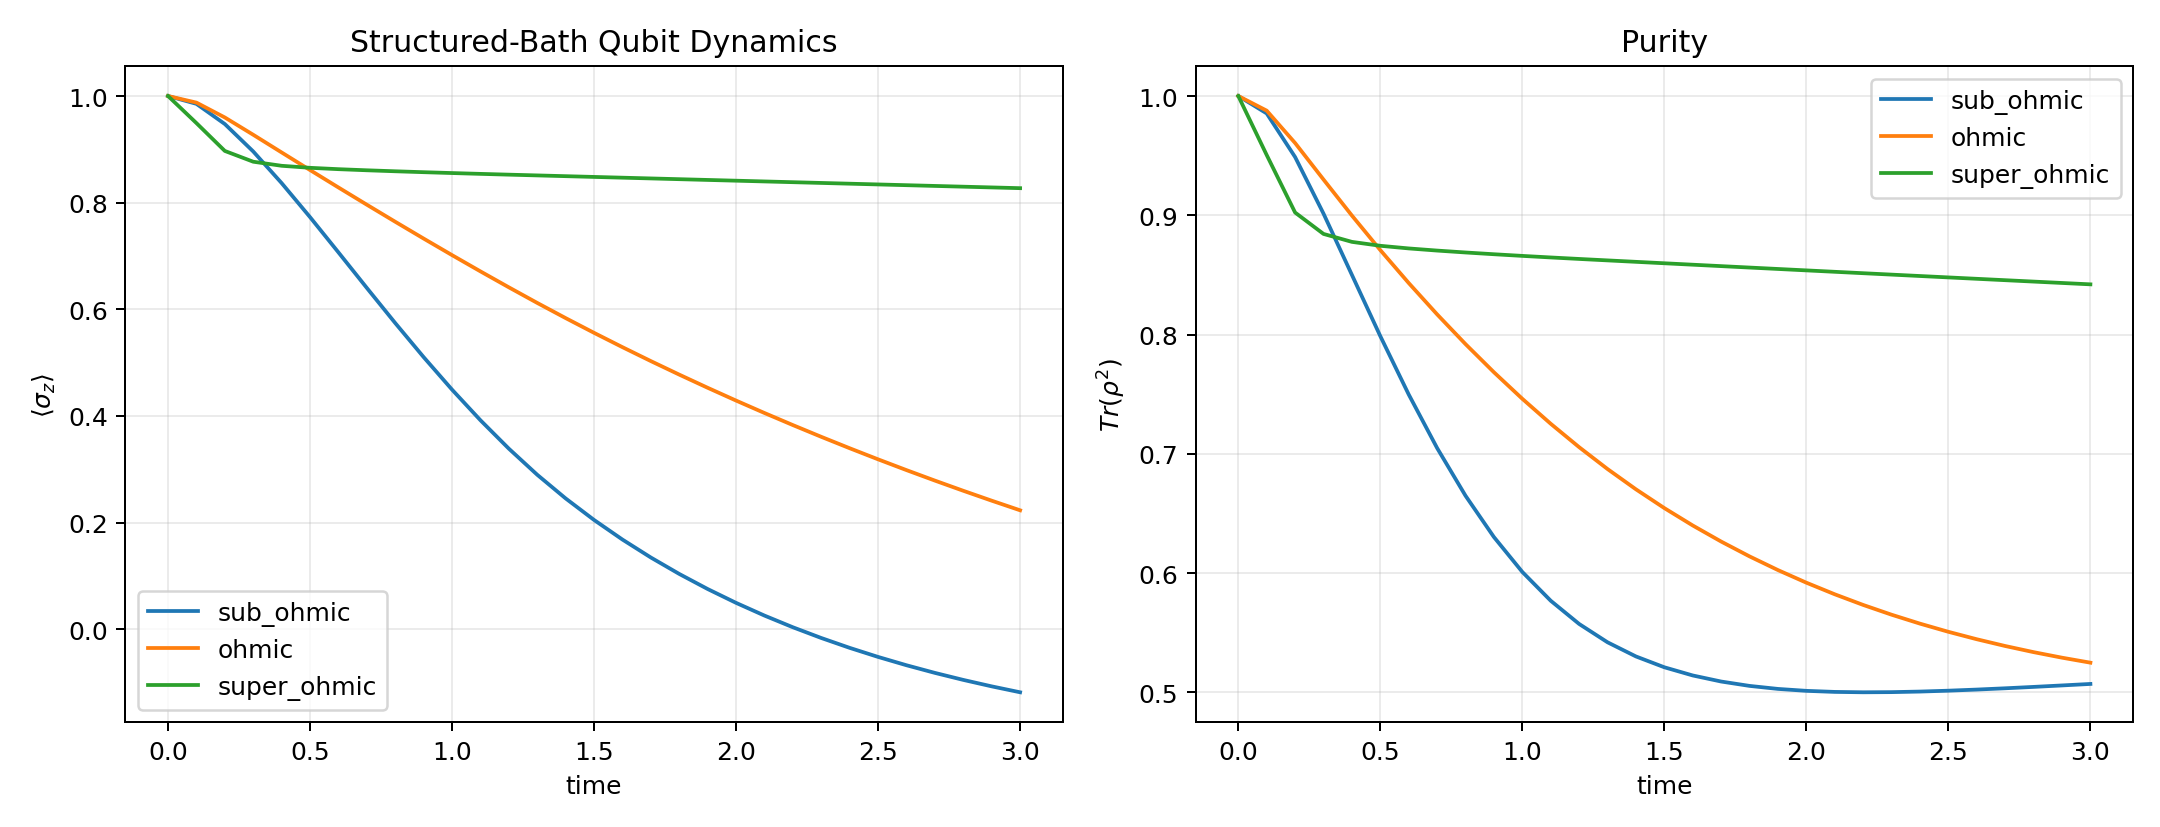
\includegraphics[width=0.74\linewidth]{single_qubit_research_regime_comparison.png}
    \caption{Reduced single-qubit dynamics for three structured-bath regimes.  This
    benchmark provides the numerical bridge between the Markovian thermal-neuron model and
    later memory-bearing gate simulations.}
    \label{fig:nonmarkovian}
\end{figure}

\section{Floquet-Buffered Reservoir Coupling}

To reduce direct exposure of the logical qubit to the reservoir, we introduce a driven
buffer between the logical subsystem and the bath,
\begin{equation}
    S \longleftrightarrow F(t) \longleftrightarrow B,
    \label{eq:buffer-architecture}
\end{equation}
and compare it with direct coupling $S\leftrightarrow B$.  A minimal buffer Hamiltonian is
\begin{equation}
    H_F(t)=\frac{\epsilon_F}{2}\sigma_z
    + A\cos(\Omega t)\sigma_x .
\end{equation}
The principal operational metric is the trace distance between two logical output states,
\begin{equation}
    D(t)=\frac{1}{2}\left\|\rho_S^{(0)}(t)-\rho_S^{(1)}(t)\right\|_1.
\end{equation}
The drive cost is monitored through the work proxy
\begin{equation}
    W_{\mathrm{drive}}
    =
    \int_0^{t_f}\mathrm{Tr}\!\left[\rho(t)\frac{\partial H_F(t)}{\partial t}\right]dt .
\end{equation}

\begin{table}[H]
\centering
\caption{Direct and Floquet-buffered logical distinguishability.}
\begin{tabular}{lrr}
\toprule
Architecture & Final trace distance & Integrated drive-work proxy \\
\midrule
Direct reservoir contact & 0.1353 & 0.0000 \\
Floquet-buffered contact & 0.1818 & 0.4604 \\
\bottomrule
\end{tabular}
\label{tab:floquet-bridge}
\end{table}

\begin{figure}[H]
    \centering
    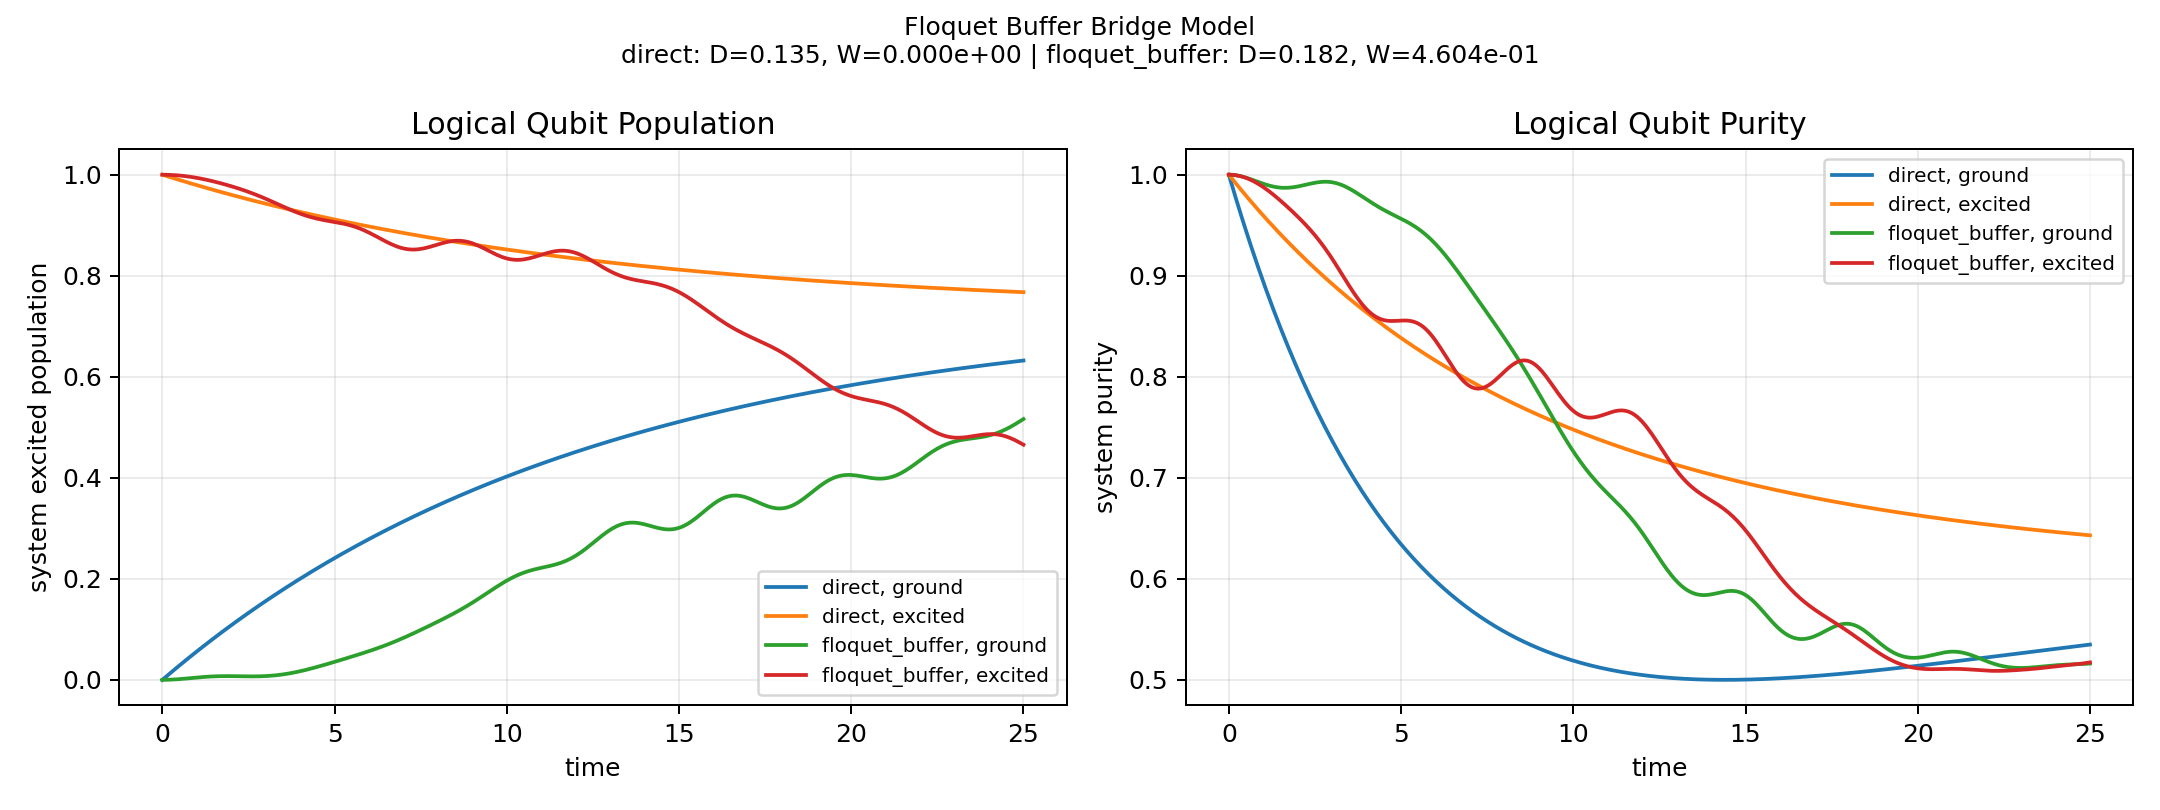
\includegraphics[width=0.74\linewidth]{floquet_buffer_comparison.png}
    \caption{Logical-qubit population and purity for direct and Floquet-buffered reservoir
    contact.  The default buffered case retains larger final distinguishability, at the cost
    of finite drive work.}
    \label{fig:floquet-bridge}
\end{figure}

\section{Parameter Screening and Gate-Prototype Decision}

A single successful Floquet-buffer run is insufficient evidence for a gate architecture.
We therefore screen the drive amplitude, drive frequency, and system-buffer coupling.  The
screening study finds positive final trace-distance gain in $14$ of $15$ tested points.  The
largest gain occurs for a weak system-buffer coupling, with
\begin{equation}
    \Delta D = 0.711315,
    \qquad
    W_{\mathrm{drive}}\approx -0.019354
\end{equation}
in the present work-proxy convention.  This value should be interpreted as a screening
indicator, not as a completed thermodynamic accounting.

\begin{figure}[H]
    \centering
    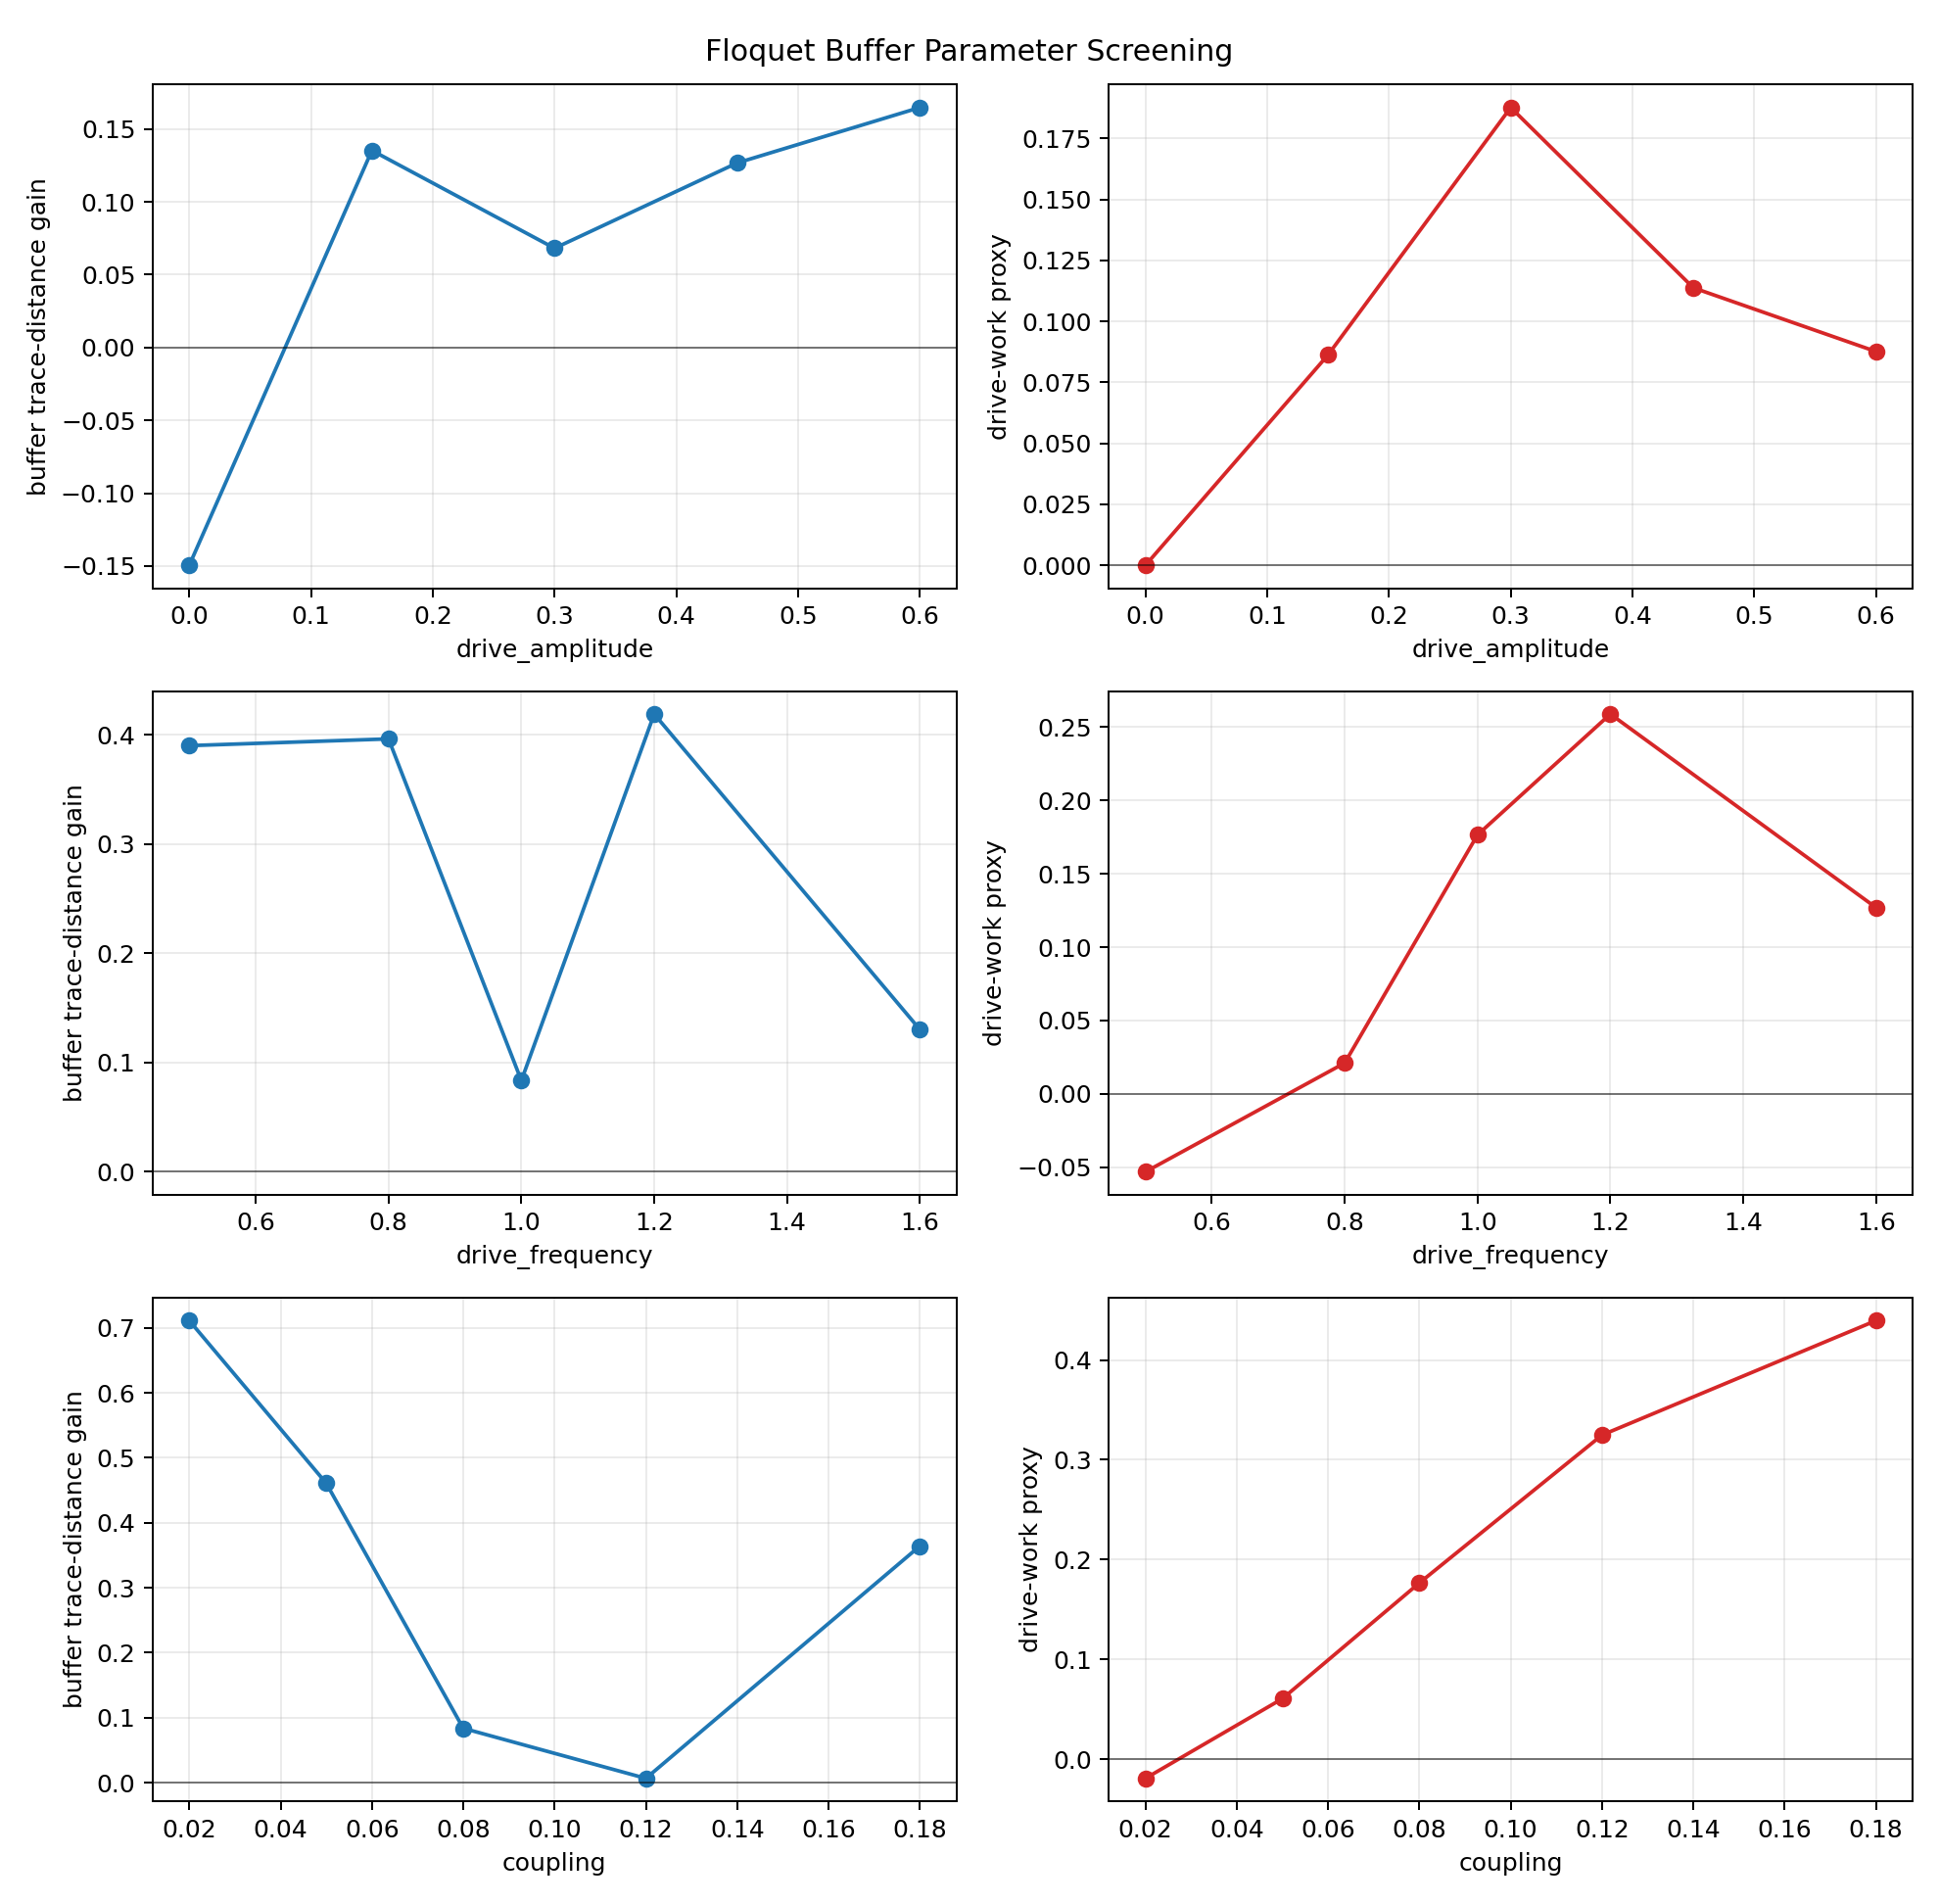
\includegraphics[width=0.78\linewidth]{floquet_parameter_sweep.png}
    \caption{Floquet-buffer parameter screening.  The buffer is assessed by the gain in
    final trace distance relative to direct reservoir contact and by the associated
    integrated drive-work proxy.}
    \label{fig:floquet-sweep}
\end{figure}

The decision analysis combines three requirements: numerical health of the non-Markovian
benchmark, positive Floquet-buffer distinguishability signal, and a baseline NOT response
sharp enough to define distinguishable logical outputs.  The resulting verdict is
\emph{risky-go}: the next simulation should be a minimal NOT-style prototype, but a full
three-qubit multi-bath gate remains premature.

\begin{figure}[H]
    \centering
    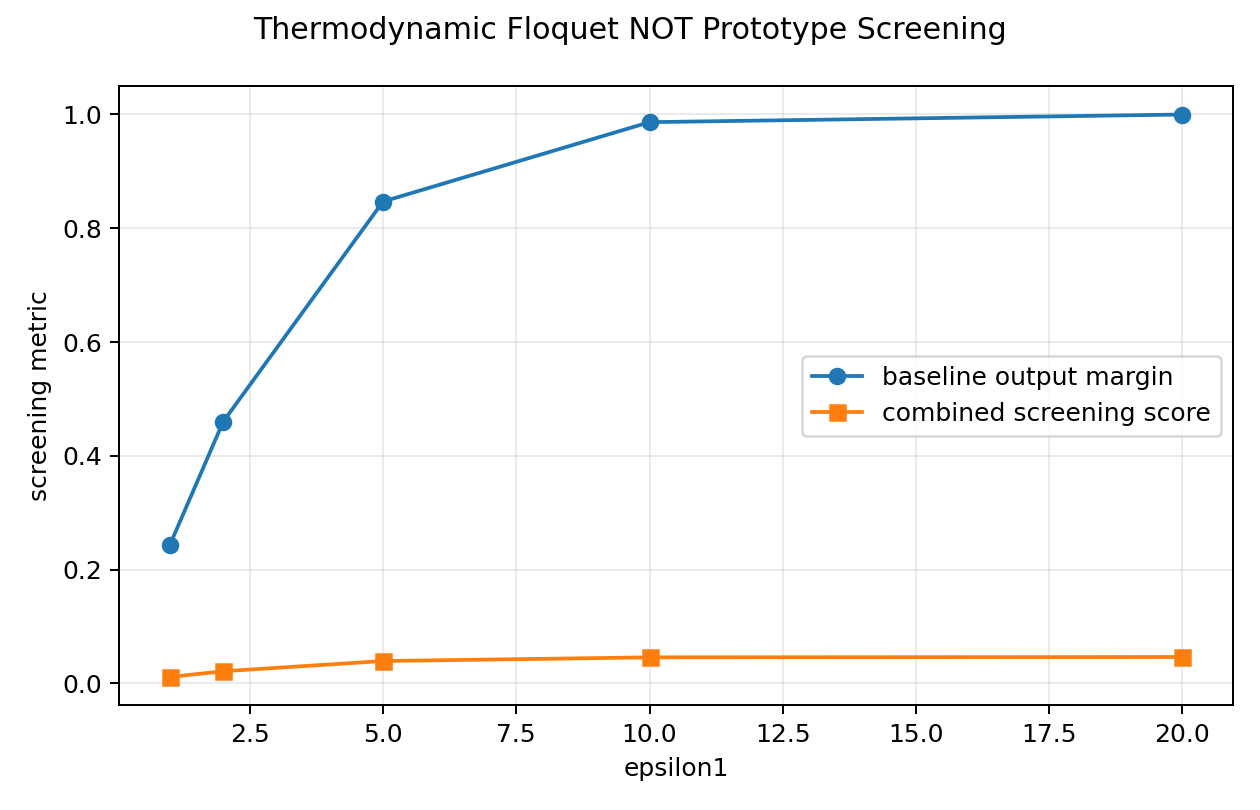
\includegraphics[width=0.74\linewidth]{not_floquet_design.png}
    \caption{Screening of NOT-gate energy scale for a Floquet-buffered prototype.  The
    largest collector energy tested gives the strongest combined score, while intermediate
    energy scales already provide usable margins for a first full-gate attempt.}
    \label{fig:not-prototype}
\end{figure}

\section{Discussion}

The results support the following interpretation.  The Markovian reset model provides a
clean thermodynamic-neuron reference: logic is obtained through virtual-temperature control
and bounded reservoir relaxation.  Increasing the collector energy scale improves logical
sharpness but increases dissipation, reproducing the expected thermodynamic trade-off.

The structured-bath benchmark indicates that the numerical machinery is stable enough for a
controlled next experiment, but it does not by itself establish a thermodynamic gate.  The
Floquet-buffer bridge adds an operationally meaningful signal: in the tested regimes, a
driven intermediate system can increase the distinguishability of logical outputs relative
to direct reservoir contact.  The correct next step is therefore not a full NOR or XOR under
multiple structured baths, but the smallest NOT-style experiment in which direct and
buffered reservoir contact are compared under the same convergence diagnostics.

\section{Conclusion}

We have reconstructed the baseline thermodynamic-neuron logic model and extended the
project to a Floquet-buffered reservoir architecture.  The reconstructed gates establish the
Markovian reference; the single-qubit structured-bath benchmark supplies numerical
stability checks; and the Floquet-buffer sweep provides a first positive screening signal
for improved logical distinguishability.  The next scientific target is a minimal
Floquet-buffered thermodynamic NOT prototype with one structured output bath.  Heat, work,
and entropy-production claims for the final non-Markovian gate should remain provisional
until interaction energy, memory effects, and external drive work are audited consistently.

\appendix
\section{Reproducibility Note}

All figures and tables in this manuscript were generated from local Python simulations.  The
main reproducibility commands are:
\begin{verbatim}
scripts/run_baseline.sh
scripts/run_non_markovian_research.sh
scripts/run_dt_convergence_scan.sh
scripts/run_memory_convergence_scan.sh
scripts/run_floquet_buffer.sh
scripts/run_floquet_buffer_sweep.sh
scripts/run_project_decision.sh
scripts/run_thermodynamic_floquet_gate_prototype.sh
\end{verbatim}
Implementation paths, generated CSV files, and run logs are intentionally kept out of the
main text so that the presentation remains in the style of a research article.

\end{document}
